\documentclass[../appunti-analisi.tex]{subfiles}

\begin{document}

\section{Lezione 25}

\subsection{Integrazione doppia su domini più generali}

Sia $D \subset \mathbb{R}^{2} $ limitato e sia $f$ limitata in $D$ ($f: D \rightarrow \mathbb{R}$)

e consideriamo l'estensione della $f$ (che chiameremo $\bar{f}$) a $D$:

\[
    \bar{f} (x,y) = \begin{cases}
        f(x,y) & \text{se $(x,y) \in D$} \\
        0 & \text{se $(x,y) \in R \setminus D $}
    \end{cases}
\]

$\bar{f} $ è in un rettangolo $R$ ed è limitata.


\defn{}{$f$ è limitata su $D \subset \mathbb{R}^{2}$ con D insieme limitato di $\mathbb{R}^{2}$.

    Diciamo che $f$ è integrabile (secondo Reimann) su D, se la $\bar{f} $ è integrabile su $R$ (secondo Reimann) e in tal caso si scrive:

    \[
        \iint_D {f(x,y)} \: d x d y = \iint_R {\bar{f} (x,y)} \: dx d y 
    \]

}

\textbf{Osservazione} 

La definizione \textbf{non} dipende dalla scelta di $R$ (dove $R$ rettagolo che contiene D)  


\defn{Insieme numerabile (Peano-Jordan)}{Un sottoinsieme limitato del piano $D \subset \mathbb{R}^{2}$ si dice misurabile (secondo Peano-Jordan) se la funzione $f(x,y)=1$ è integrabile su D 

In tal caso poniamo:

\[
    Area(D) = \underbrace{|D|}_\text{area} = \iint {1} \: dx d y
\]

e dunque ogni rettangolo $R = [a,b] \times [c,d]$ è misurabile secondo Peano-Jordan:

\[
    |R| = \int_{a}^{b} {\int_{c}^{d} {1} \: dx } \: dx  = (b-a) (d-c)
\]
}


Tutti gli insiemi che conosciamo della geometria elementare (quadrati, rettangoli, poligoni, cerchi) sono misurabili e la loro misura (secondo Peano-Jordan) è l'area che conosciamo:

\[
    Q = [0,1] \times [0,1]
\]

quadrato con le componenti razionali:

\[
    f() = \begin{cases}
        1 & \text{se $(x,y) \in Q$ e $(x,y)$ razionali} \\
         0 & \text{altrimenti}
    \end{cases}
\]

non è Riemann integrabile.


\subsubsection{Proprieta}

Siano $f$ e $g$ integrabili su D ( siano $f,g \in R(D)$) e $c \in \mathbb{R}$:

\begin{enumerate}
    \item Linearita'
        \begin{enumerate}
            \item $f+g$ è integrabile:

                \[
                    \iint_D {(f+g)} \: dx d y  = \iint_D {f} \: dx d y + \iint_D {g} \: dx d y 
                \]
            \item $c\cdot f$ è integrabile:

                \[
                    \iint_D {c f()} \: dx  d y = c \iint_D {f()} \: dx  d y 
                \]

            \item \[
                \iint_D {[\alpha f() + \beta g() } \: dx d y = \alpha \iint_D {f()} \: dx d y + \beta \iint_D {g()} \: dx d y 
            \]
        \end{enumerate}

    \item Monotonia
        \begin{enumerate}
            \item Se $f \le g$ allora:

                \[
                    \iint_D {f()} \: dx d y \le  \iint_D {g()} \: dx d y 
                \]
            \item $|f| \in R(D)$ e si ha $\left|\iint_D {f()} \: dx d y \right| \le \iint_D {\left|f()\right|} \: dx d y  $

                In particolare se $D$ è misurabile e se $M_1= \underbrace{sup}_\text{D} | f(x,y)|$:

                \[
                    \left|\iint_D {f(x,y)} \: dx d y\right| \le M_1(D)
                \]

        \end{enumerate}
        
\end{enumerate}


\newpage 

\subsection{Regioni semplici del piano}

Sono insiemi misurabili (secondo Peano-Jordan) e su queste regioni possiamo usare le formule di riduzione.

Una regione $D_1 \subset \mathbb{R}^{2}$ si dice \textbf{y-semplice} (o normale rispetto all'asse x) se è compresa tra i grafici di due funzioni della variabile x.

\textbf{Esempio} 

DISEGNO DA FARE

\[
    D_1= \{(x,y) \in \mathbb{R}^{2}, a \le x \le b, g_1(x) \le y \le g_2(x)\}
\]

dove $g_1,g_2$ sono continue in $[a,b]$ e $g_1(x) \le g_2(x)$.

$D_1$ è l'insieme di segmenti verticali se $x \in [a,b]$

\[
    (D_1)x = \{y \in \mathbb{R}, g_1(x) \le y \le g_2(x)\} = \begin{cases}
        [g_1(x),g_2(x)] & \text{se $x \in [a,b]$} \\
        \emptyset & \text{altrimenti}
    \end{cases}
\]

$D_2$ è \textbf{x-semplice} (normale rispetto all'asse y)

DISEGNO DA FARE


\[
    D_2= \{(x,y) \in \mathbb{R}^{2}, c \le y \le d, h_1(y) \le x \le h_2(y)\}
\]
 
dove $h_1,h_2$ sono continue $[c,d]$ e $h_1(y) \le h_2(y)$.

$D_2$ è l'insieme di segmenti orizzontali:

\[
    (D_2) y = \{x \in \mathbb{R}, h_1(y) \le x \le h_2(y)\} = \begin{cases}
        h_1(y),h_2(y) & \text{se $y \in [c,d]$} \\
        \emptyset & \text{altrimenti}
    \end{cases}
\]


$D_1$ e $D_2$ sono misurabili secondo Peano-Jordan.

\[
    Area(D_1) = \int_{a}^{b} {[g_2(x) -g_1(x)]} \: dx 
\]

cioe':

\[
    \iint_{D_1} {1} \: d x d y = \int_{a}^{b} {dx \int_{g_1(x)}^{g_2(x)} {1} \: d y }
\]

mentre:

\[
    Area(D_2) = \int_{c}^{d} {[h_2(x) -h_1(x)]} \: dx 
\]

cioe':

\[
    \iint_{D_2} {1} \: d x d y = \int_{c}^{d} {dx \int_{h_1(x)}^{h_2(x)} {1} \: d y }
\]


\teorema{Formule di riduzione}{ Ogni funzione continua su un'insieme semplice $D \subset \mathbb{R}^{2}$ è integrabile su tale insieme e valgono le formule di riduzione:

    \begin{enumerate}
        \item Se $D$ è y-semplice allora:

            \[
                \iint_D {f(x,y)} \: d x d y = \int_{a}^{b} {d x \int_{g_1(x)}^{g_2(x)} {f(x,y)} \: d y } 
            \]
        \item Se $D$ è x-semplice allora:

            \[
                \iint_D {f(x,y)} \: d x d y = \int_{c}^{d} {d y \int_{h_1(y)}^{h_2(y)} {f(x,y)} \: d x } 
            \]
    \end{enumerate}

}

\textbf{Esempio} 

Dato:

\[
    E = \{(x,y) \in \mathbb{R}^{2}| 0 \le x \le 2, -x \le y \le x^{2}\}
\]

Rappresentarlo come insieme x-semplice (o come unione di insiemi x-semplici)


DISEGNO DA FARE


x-semplice unione di segmenti orizzontali

\[
    E = \{(x,y) \in \mathbb{R}^{2}; -2 \le y \le 0, \underbrace{-y}_\text{$h_1(y)$} \le x \le \underbrace{2}_\text{$h_2(y)$}\} \cup \{(x,y) \in \mathbb{R}^{2}; 0 \le y \le 4, \underbrace{\sqrt{y}}_\text{$g_1(x)$} \le  x \le \underbrace{2}_\text{$g_2(x)$}\}
\]


DISEGNO

$D_1$ è y-semplice.

$D_2$ è x-semplice.

$D = D_1 \cup D_2$ non è semplice

\[
    \iint_D {f()} = \iint_{D_1} {f()} + \iint_{D_2} {f()}
\]

\subsubsection{Proprietà di additività rispetto ai domini di integrazione}

Supponiamo che $D_1,D_2,\ldots,D_k \in \mathbb{R}^{2}$ sono semplici e che non abbiamo due a due punti in comune oltre ad una parte di frontiera allora ogni funzione continua in $D = D_1 \cup \ldots \cup D_k$ è integrabile e:

\[
    \iint_D {f(x,y)} \: d x d y = \iint_{D_1} {f(x,y)} \: d x d y + \ldots + \iint_{D_k} {f(x,y)} \: d x d y  
\]

\newpage

\textbf{Esempio}

\[
    \int_{0}^{1} {\int_{x}^{1} {e ^{y^{2}}} \: dy } \: dx 
\]

\begin{itemize}
    \item y-semplice
        \[
            D = \{(x,y) \in \mathbb{R}^{2}, 0 \le x \le 1, x \le y \le 1\}
        \]
    \item x-semplice
        \[
            D = \{(x,y) \in \mathbb{R}^{2}, 0 \le y \le 1, 0 \le x \le y\}
        \]
\end{itemize}

\[
    \iint_D {e ^{y^{2}}} \: d y d x = \int_{0}^{1} {\left(\int_{x}^{1} {e ^{y^{2}}} \: d y \right)} \: dx = \int_{0}^{1} {\left(\int_{0}^{y} {e ^{y^{2}}} \: dx \right)} \: d  y = \int_{0}^{1} {e ^{y^{2}}\left(\int_{0}^{y} {} \: dx \right)} \: dy  =
\]

\[
    = \int_{0}^{1} {y e ^{y^{2}}} \: dy  = \Eval{[\frac{1}{2} e ^{y^{2}}]}{0}{1} = \frac{1}{2} (2 -1) = -\frac{1}{2}
\]

dove $\int_{0}^{1} {\left(\int_{x}^{1} {e ^{y^{2}}} \: dy \right)} \: dx $ è una funzione continua e dunque ammette primitiva $F(y)$ quindi otteniamo:

\[
    \int_{0}^{1} {\left(\int_{x}^{1} {e ^{y^{2}}} \: dy \right)} \: dx  = \int_{0}^{1} {\Eval{[F(y)]}{x}{1} } \: dx = \int_{0}^{1} {\left(F(1) - F(x) \right)} \: dx =
\]

\[
    = \int_{0}^{1} {F(1)} \: d x - \int_{x}^{1} {F(x)} \: dx = F(1) - \int_{0}^{1} {F(x)} \: dx  =
\]

\[
    = F(1) - \Eval{[xF(x)]}{0}{1} + \int_{0}^{1} {x F'(x)} \: dx = \cancel{F(1)} \cancel{- F(1)} + 0 + \int_{0}^{1} {xF'(x)} \: dx
\]

\[
    = \underbrace{\int_{0}^{1} {x e^{x^{2}}} \: dx }_\text{risultato come sopra}
\]

\subsection{Cambiamento di variabili degli integrali doppi (non la spiega in realta boh)}

In analisi I, abbiamo utilizzato il \textbf{metodo della sostituzione}:

$x$ e $t$ allora $x=\varphi(t)$, dove $\varphi$ è $\mathbb{C}^{1}$ ed invertibile:

\[
    \int_{a}^{b} {f(x)} \: dx = \int_{\varphi^{-1}(a)}^{\varphi^{-1}(b)} {f(\varphi(t))\varphi'(t)} \: dt 
\]

dove $d x = \varphi'(t) dt$


\subsection{Integrali doppi in coordinate polari}

Consideriamo l'applicazione (vettore): $F: \mathbb{R}^{2} \rightarrow \mathbb{R}$ cosi definita:

\[
    (\rho, \theta) \rightarrow (\underbrace{x(\rho, \theta)}_\text{$F_1(\rho, \theta)$}, \underbrace{y(\rho, \theta)}_\text{$F_2(\rho,\theta)$})
\]

\[
    F = \begin{cases}
        x=\rho \cos \theta\\
         y = \rho \sin \theta
    \end{cases}
\]


Consideriamo la matrice Jacobiana associata a $F(2\times 2 )$

\[
    DF(\rho,\theta) = JF(\rho,\theta)
\]

\[
    DF(\rho,\theta) = JF(\rho,\theta) = \begin{vmatrix}
    \nabla F_1(\rho,\theta)\\
     \nabla F_2(\rho,\theta)
    \end{vmatrix} = \begin{vmatrix}
    \frac{\partial F_1}{\partial \rho}(\rho,\theta) & \frac{\partial F_1}{\partial \theta}(\rho,\theta)\\
    \frac{\partial F_2}{\partial \rho}(\rho,\theta) & \frac{\partial F_2}{\partial \theta}(\rho,\theta)
    \end{vmatrix} = \begin{vmatrix}
    \cos \theta & \rho \sin \theta\\
    \sin \theta & \rho \cos \theta 
    \end{vmatrix}
\]

calcoliamo il determinante:

\[
    det JF(\rho,\theta) = \rho \cos^{2}\theta+ \rho \sin^{2}\theta = \rho \neq 0 \Leftrightarrow \theta \neq 0
\]

Quindi $\rho=0 \Leftrightarrow (x,y) = (0,0)$

La funzione $F$ non è iniettiva (non c'è corrispondenza 1 a 1) per la periodicita' delle funzioni trigonometriche:

\[
    F(\rho, \theta + 2\pi) = F(\rho,\theta) = (\rho \cos (\theta+ 2\pi), \rho \sin (\theta + 2\pi) + \text{ valori associati}
\]

Restringiamo la funzione $F$ ad $A \subset \mathbb{R}^{2}$ aperto in cui:

\[
    A = (0, +\infty) \times (0, 2\pi) \text{ oppure } A=(0, +\infty) \times (-\pi, \pi)
\]

quindi l'applicazione:

\[
    F: A \subseteq \mathbb{R}^{2} \rightarrow \mathbb{R}
\]

è biettiva perché manda aperti in aperti.

\newpage

\begin{figure}
 \centering
 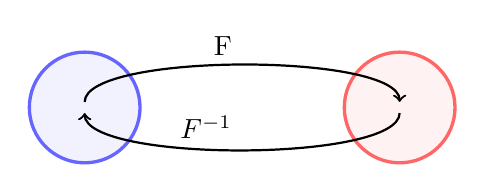
\begin{tikzpicture}[
     ele/.style={fill=black,circle,minimum width=.8pt,inner sep=1pt},every fit/.style={ellipse,draw,inner sep=-2pt},
     insieme/.style={circle, draw=blue!60, fill=blue!5, very thick, minimum size=40},
     insiemeLel/.style={circle, draw=red!60, fill=red!5, very thick, minimum size=40},
     ]
  \node[insieme] (a1) at (0,4) {};    
  % \node[ele,label=left:$c$] (a3) at (0,2) {};
  % \node[ele,label=left:$d$] (a4) at (0,1) {};

  \node[insiemeLel] (b1) at (4,4) {};
  % \node[ele,,label=right:$3$] (b3) at (4,2) {};
  % \node[ele,,label=right:$4$] (b4) at (4,1) {};


  \draw[->,thick,shorten <=2pt,shorten >=2pt] (b1.center) .. controls +(down:7mm) and +(down:7mm) .. (a1.center) node[midway,above left] {$F^{-1}$};
  \draw[->,thick,shorten <=2pt,shorten >=2] (a1.center) .. controls +(up:7mm) and +(up:7mm) .. (b1.center) node[midway,above left] {F};
  % \draw[->,thick,shorten <=2pt,shorten >=2] (a2) -- (b2) node[midway,above left] {F};
  % \draw[->,thick,shorten <=2pt
  % \draw[->,thick,shorten <=2pt,shorten >=2] (b2) -- (a2) node[midway,above left] {$F^{-1}$};
  % \draw[->,thick,shorten <=2pt,shorten >=2] (a4) -- (b3);
 \end{tikzpicture}
\label{fig:polari}
\caption{Funzione per le coordinate polari invertibile}
\end{figure}


\teorema{}{Consideriamo l'applicazione verticale $F(\rho,\theta) = \left(F_1(\rho,\theta), F_2(\rho,\theta)\right)$ in cui $F: A \rightarrow \mathbb{R}^{2}$ in cui $A = (0,+\infty) \times (0,2\pi)$.

    Sia $S \subset (0,+\infty) \times (0,2\pi)$ un aperto misurabile nel piano $(\rho,\theta)$ con $\bar{S} \subset (0,\infty) \cdot (0,2\pi)$ e sia $T=F(S)$ (fig. \ref{fig:polari})


Allora per ogni funzione $f$ integrabile su $T$, continua e limitata, vale la sequente formula:

\[
    \iint_{T=F(S)} {f(x,y)} \: d x d y  = \iint_{S=F'(T)} {f( \rho \cos \theta, \rho \sin \theta) \underbrace{\rho}_\text{det $JF(\rho,\theta)$}} \: d \rho d \theta  
\]

}


% \textbf{Esempio} 
%
% Cerchio: $x^{2}+y^{2}=r^{2}$
%
% Coordinate polari:
%
% \[
%     \{(\rho,\theta) | 0 \le \rho \le r, 0 \le \theta \le  2\pi\}
% \]
%
% \[
%     c = \{(x,y) \in \mathbb{R}^{2}| r^{2} \le x^{2}+y^{2} \le R^{2}\}
% \]
%
% \[
%     \bar{c} = \{(\rho,\theta) | r \le \rho \le R, 0 \le \theta \le 2\pi\}
% \]
%
% DISEGNI SU DISEGNI CHE BELLO


\textbf{Esempio} 

\[
    \iint_{u^{2}+v^{2} \le S} {v^{2}} \: dudv 
\]

\[
    D= \{(u,v) \in \mathbb{R}^{2}, u^{2}+v^{2} \le S\}
\]

Trasformiamo in coordinate polari (in questo caso ha senso perché la forma di A è un cerchio, in casi come questo conviene usare le coordinate polari):

\[
    \bar{D} = \{(\rho,\theta) | 0 \le \rho \le \sqrt{5}, 0 \le \theta \le 2\pi\}
\]

\[
    \iint_{u^{2}+v^{2} \le S} {v ^{2}} \: dudv = \int_{0}^{\sqrt{5}} {\int_{\theta}^{2\pi} {\rho^{2} \sin \theta \cdot \rho} \: d \rho } \: d \theta = \int_{0}^{\sqrt{5}} {\int_{\theta}^{2\pi} {\theta^{3} \sin \theta} \: d \theta } \: d \rho =  
\]

\[
    \int_{0}^{\sqrt{5}} {\rho^{3} \left(\int_{\theta}^{2\pi} {\sin ^{2} \theta} \: d \theta \right)} \: d \rho = \int_{0}^{\sqrt{5}} {\rho^{3} \left( \int_{\theta}^{2\pi} { \frac{1- \cos 2 \theta}{2}} \: d \theta \right)} \: d \rho =   
\]

\[
    = \int_{0}^{\sqrt{5}} {\rho^{3} \Eval{[ \frac{1}{2} \theta - \frac{\sin 2 \theta}{4}]}{0}{2\pi} } \: d \rho = \pi \int_{0}^{\sqrt{5}} {\rho^{3}} \: d \rho  = \pi \Eval{[ \frac{\rho^{4}}{4}]}{0}{\sqrt{5}}  = \frac{25}{4}\pi 
\]

\textbf{Esempio} 

\[
\iint_A {x^{2}+y^{2}} \: d x d y  
\]

\[
    A = \{(x,y) \in \mathbb{R}^{2} | x^{2} + y^{2} \le 4\}
\]

\[
    A = \underbrace{\{(x,y) \in \mathbb{R}, -2 \le x \le 2, - \sqrt{4-x^{2}} \le  y \le  \sqrt{4 -x^{2}}\}}_\text{dominio y-semplice}\]

Vediamo il metodo lungo (complicato che non va bene):
\[
    \iint_A {x^{2}+y^{2}} \: d x d y = \int_{-2}^{2} {} \: dx  \int_{-\sqrt{4-x^{2}}}^{\sqrt{4-x^{2}}} {\left(x^{2} + y^{2}\right)} \: d y  = \int_{-2}^{2} { \Eval{[x^{2}(y)+ \frac{y^{3}}{3}]}{-\sqrt{4-x^{2}}}{\sqrt{4-x^{2}}} } \: dx 
\]

ora passiamo in coordinate polari invece per facilitarci:

\[
    \bar{A}  = \{(\rho,\theta) | 0 \le \rho \le 2, 0 \le \theta \le 2\pi\}
\]

\[
    \iint_A {x^{2}+y^{2}} \: d x d y = \int_{0}^{2} {\int_{0}^{2\pi} {\theta^{2} \rho} \: d \rho } \: d \theta = 2\pi \int_{0}^{2} {\rho^{3}} \: d \rho = 2\pi \Eval{[ \frac{\rho^{4}}{4}]}{0}{2} = 2\pi 
\]

\textbf{Esempio} 

\[
\iint_A {x} \: dx d y; \iint {y} \: d x d y  
\]

\[
    A = \{(x,y) \in \mathbb{R}^{2} | x^{2}+y^{2} \le 1, x>0\}
\]

\[
    \iint_A {y} \: d x d y =0 
\]

la funzione integranda:

\[
    f(x,y) = y, f(x,-y) = -y
\]

\[
    \bar{A} = \{(\rho,\theta) | 0 \le \theta \le 1, - \frac{\pi}{2} \le \theta \le \frac{\pi}{2}\}
\]

\[
    \iint_A {x} \: d x d y  = \int_{0}^{1} {\int_{- \frac{\pi}{2}}^{ \frac{\pi}{2}} {\rho \cos \theta \rho} \: d \rho } \: d \theta = \int_{0}^{1} {\rho^{2} \left(\int_{- \frac{\pi}{2}}^{ \frac{\pi}{2}} {\cos \theta} \: d \theta \right)} \: d \rho =  
\]

\[
    =\int_{0}^{1} {\rho^{2}\Eval{[\sin \theta]}{ - \frac{\pi}{2}}{ \frac{\pi}{2}} } = 2 \int_{0}^{1} {\rho^{2}} \: d \rho = \Eval{[2 \frac{\rho^{3}}{3} ]}{0}{1} = \frac{2}{3}
\]

\end{document}
